\documentclass[12pt]{article}

% preamble
\usepackage{amsmath}
\usepackage[margin = 1in]{geometry}
\usepackage{graphicx}
\usepackage{booktabs}
\usepackage{natbib}

% highlighting hyper links
\usepackage[colorlinks=true, citecolor=blue]{hyperref}

\title{Comparison of Multi-Class Classification Methods}
\author{Sean Murphy\\
  Statistics Major\\
  University of Connecticut
}

\begin{document}
\maketitle

\begin{abstract}
THE ABSTRACT WILL BE WRITTEN AFTER THE REST OF THE PAPER HAS BEEN WRITTEN. 
\end{abstract}

\section{Introduction}
\label{sec:intro}

% Use this section to answer three questions:
% Why is the topic important/interesting?
% What has been done on this topic in the literature?
% What is your contribution?

The rest of the paper will be organized in the following way.  
An introduction to the red wine data set will be presented in 
Section~\ref{sec:data}.  This section will describe the variables 
and observations contained in the dataset, and will include a brief 
overview of summary statistics.  Next, a methodological overview of 
this analysis will be given in Section~\ref{sec:meth}.  Each of the 
classification methods and their underlying assumptions will be 
presented in Section~\ref{sec:class}.  The classification metrics 
which will be used to compare the predictive effectiveness of each 
model will be introduced in Section~\ref{sec:metr}.  After this, 
the results will be presented with tables and figures in 
Section~\ref{sec:resu}.  Finally, once the results of the analysis 
have been described, a discussion of their implications and 
suggestions for further study will be covered in Section~\ref{sec:disc}.


\section{Data}
\label{sec:data}

The data that will be analyzed in this study comes from the UC Irvine Machine 
Learning Repository.  It is a dataset from 2009 containing information about 
a sample of red "Vinho Verde" wine from north Portugal.  The dataset contains 
$n = 1,599$ observations (different wine samples) of twelve variables, eleven 
of which are continuous numeric variables.  These continuous variables are 
different physiochemical measurements of the wine samples: fixed acidity, 
volatile acidity, citric acid, residual sugar, chlorides, free sulfur dioxide, 
total sulfur dioxide, density, pH, sulfates and alcohol.  The other variable 
contained in the dataset is wine quality, which takes integer values from 0-10 
(0 being lowest quality, 10 being highest quality).  Though numeric, this 
variable will be treated as having 11 classes, and will be the response variable 
in the analysis.  The goal is to predict the class of wine quality for a given 
sample of red wine based on its physiochemical properties.  

PROVIDE HERE SOME SUMMARY STATISTICS OF THE DATASET

See a summary of the counts of wine samples at each quality level in 
Table~\ref{tab:qual}.

We can see that there are no wine samples in our dataset that had quality 
levels of 0, 1, 2, 9, or 10.  All of the quality levels fell within the 
range from 3 to 8, and within this range, the vast majority were rated 
either a 5 or a 6.  Indeed, these two levels alone account for over 82 
percent of the data.  

We can see in the histogram and boxplot in Figure~\ref{fig:wine} that 
the distribution of wine quality levels is roughly symmetric, with 
outliers depicted in the boxplot at quality levels of 3 and 8.  

\begin{table}[tbp]
 \caption{This table provides the number of wine samples by each wine quality level.}
\label{tab:qual}
\centering
\begin{tabular}{rrr}
 \toprule
 Quality Level & Count \\ 
 \midrule
0 & 0 \\ 
1 & 0 \\ 
2 & 0 \\ 
3 & 10 \\ 
4 & 53 \\ 
5 & 681 \\ 
6 & 638 \\ 
7 & 199 \\ 
8 & 18 \\ 
9 & 0 \\ 
10 & 0 \\
\bottomrule
\end{tabular}
\end{table}

\begin{figure}[tbp]
 \centering
 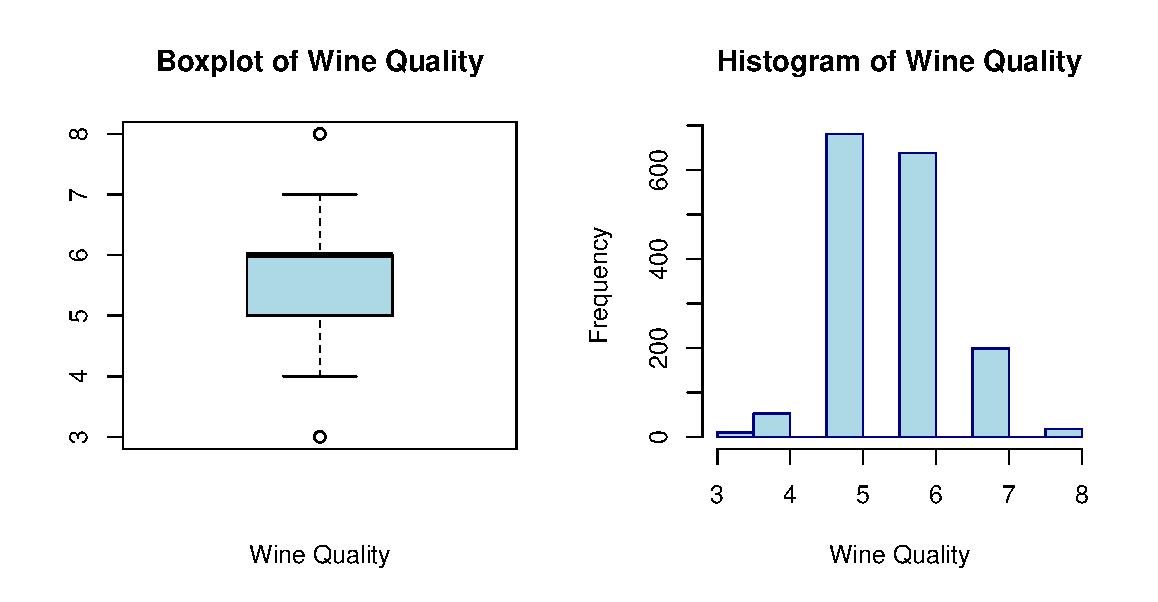
\includegraphics[width=\textwidth]{manuscriptfigure.pdf}
 \caption{A boxplot and a histogram of the wine quality for the samples of Portuguese red wine.}
 \label{fig:wine}
\end{figure}

\section{Methods}
\label{sec:meth}

OVERVIEW PARAGRAPH

\subsection{Classification Methods}
\label{sec:class}

MULTINOMIAL LOGISTIC REGRESSION

In classification, multinomial regression is the name given to the 
logistic regression model that predicts response variable values for 
$K > 2$ classes.  Since it is an extension of logistic regression for 
binary classification, it shares many of the same characteristics.  
Logistic regression models in general are modifications to linear 
regression models that make them fit to return values between 0 and 1.  
Recall that a multiple linear regression model takes the following form:
\begin{equation}
  \label{eq:linreg}
  Y = \beta_0 + \beta_1X_1 + ... + \beta_pX_p + \epsilon.
\end{equation}
In Equation~\eqref{eq:linreg}, we see that there is nothing restricting 
$Y$ from taking values $> 1$ or $< 0$.  This is problematic if we wish 
for our model to predict the probability that the response variable 
falls within a particular class, since probabilities can only take 
values between 0 and 1.  In order to solve this problem, the binary 
classification logistic regression model takes the following form:
\begin{equation}
  \label{eq:logreg}
  p(X) = 
  \frac{e ^ {\beta_0 + \beta_1X_1 + ... + \beta_pX_p}} 
  {1 + e ^ {\beta_0 + \beta_1X_1 + ... + \beta_pX_p}}.
\end{equation}
In Equation~\eqref{eq:logreg}, we see that this problem is essentially 
solved by exponentiation.  The multiple linear regression model is 
placed into the exponent of $e$ to ensure that the numerator and 
denominator will always be positive.  This means that the overall 
model will not return values $< 0$.  Additionally, because the numerator 
will never exceed the denominator, the fraction will always be $\leq 1$.  
Thus, the model outputs values in the desired range for predicting probabilities. 
 Since in binary classification there are only two classes, the output of 
 this model represents the probability that $Y$ will fall into one of the 
 predetermined classes.  The probability that $Y$ will fall into the other 
 class is simply $1 - p(X)$.

 In multinomial logistic regression, however, there are more than 2 classes 
 into which the response variable could fall.  The binary model is generalized 
 to $K > 2$ classes in the following manner:
 \begin{equation}
  \label{eq:multireg}
  Pr( Y = k | X = x ) = 
  \frac{e ^ {\beta_k0 + \beta_k1X_1 + ... + \beta_kpX_p}}
  { \sum_{l = 1} ^ {K}  e ^ {\beta_l0 + \beta_l1X_1 + ... + \beta_lpX_p}},
\end{equation}
where $x$ is a vector of the $p$ predictor values.  In 
Equation~\eqref{eq:multireg}, we see that the numerator is the exponentiated 
linear model for class $k$, while the denominator is the sum of the 
exponentiated linear models for all $K = k$ classes.  It should be noted 
that this is not the only way of generalizing the binary logistic regression 
model to $K >2$ classes.  The model presented in Equation~\eqref{eq:multireg} 
is known as the \textit{softmax} coding \citep{james2021introduction}.  
There are other versions of multinomial regression models, but we will not 
use them and thus not elaborate on them further for this analysis.  

Among the most notable assumptions for the logistic regression model are 
the linear decision boundary and the independence of the predictors used 
in the model \citep{khan2023comparison}.

\subsubsection{Generative Models}
\label{sec:gm}

OVERVIEW PARAGRAPH

The next three multi-class classification methods are very similar in structure, 
and so it will be useful to introduce their shared underlying methodology before 
discussing their peculiarities.  In multinomial logistic regression, the approach 
is to attempt to model $Pr( Y = k|X = x)$ directly.  However, there is an 
alternative approach that can prove more useful in certain circumstances.  This 
approach is to employ Bayes' Theorem, which obtains $Pr( Y = k | X = x)$ indirectly 
by first obtaining the conditional distribution of $X$ in each class, $K$, and then 
using these distributions to obtain the desired probability that $Y$ will fall into 
$k$ given some vector of predictors $x$.  The general model takes the following form:
\begin{equation}
  \label{eq:genmod}
  Pr(Y = k | X = x) =
  \frac{\pi_k f_k(x)} {\sum_{l = 1} ^ {K} \pi_l f_l(x)}
\end{equation}
In Equation~\eqref{eq:genmod}, the $\pi_k$ term in the numerator simply is the prior 
probability that $Y$ falls into class $k$.  This is computed by the proportion of all 
the observations in the sample that fall into the $k ^ {th}$ class.  The $f_k(x)$ term 
describes the conditional distribution of $X$ in class $k$.  In other words, 
$f_k(x) = Pr(X = x | Y = k)$.  These two numerator terms are divided by the same two 
terms for each class $k$ summed in the denominator.  That is, the denominator contains 
the sum of the prior probabilities that $Y$ will fall into each of the $K$ classes 
multiplied by the corresponding conditional distribution of $X$ in that class.  Thus, 
the general form of the generative model is simply Bayes' Theorem, which returns here 
an estimate of the probability that $Y$ will fall into class $k$ given some vector of 
predictors.  

Each of the next three multi-class classification models that we will consider is some 
variant of the above, and they are principally differentiated by their varying strategies 
for approximating $f_k(x)$.  The three kinds of generative models that we will consider 
in this paper are linear discriminant analysis (LDA), quadratic discriminant analysis 
(QDA), and naive Bayes (NB).  We will discuss each of them in turn.  

LINEAR DISCRIMINANT ANALYSIS

Linear Discriminant Analysis (LDA) is a generative model that approximates $f_k(x)$ by 
assuming that each of the predictors comes from a normal distribution.  In the case of 
multiple predictors such as we have in this analysis, this means that LDA assumes $x$ 
(the vector of $p$ predictors) follows a multivariate normal distribution.  The mean, 
$\mu$, of this multivariate normal distribution is a vector containing the mean value 
of each predictor.  The covariance of the predictors, $\Sigma$, is the $p$ by $p$ 
covariance matrix of the vector $x$.  Therefore, we can say in shorthand that 
$x ~ N(\mu,\Sigma)$.  Thus, since the conditional distribution of the vector $x$ in 
each class $k$ is assumed to be multivariate normal, the density function is 
$$Pr(X = x|Y = k) = \frac {1} {(2\pi) ^ {p/2} |\Sigma| ^ 
{1/2}} exp(-\frac{1}{2}   (x - \mu_k) ^ T \Sigma ^ {-1} (x - \mu_k))$$.  
Here, $\mu_k$ is simply the vector of the mean values of the $p$ predictors where 
$Y = k$, and $\Sigma$ is the common covariance matrix of $x$ for each of the $k$ 
classes.  The above equation can then be plugged into Equation~\eqref{eq:genmod} 
for $f_k(x)$, the resulting equation of which we will not reproduce here because of 
its complexity.  Suffice it to say that this equation now obtains for us the probability 
that $Y$ falls in class $k$ given a particular vector of predictors $x$, so that the 
model gives the value for $Pr(Y = k|X = x)$.

In order to classify a vector of predictors $x$ to some class $Y = k$, we look for the 
class in which the value of the above $Pr(Y = k|X = x)$ is greatest.  With some 
algebraic rearrangement, this is equivalent to classifying a vector $x$ to the 
class for which the following equation is greatest:
\begin{equation}
  \label{eq:disscore}
  \delta_k(x) = x ^ T \Sigma ^ {-1} \mu_k - 
  \frac {1} {2} \mu_k ^ T \Sigma ^ {-1} \mu_k + \log {\pi_k}
\end{equation}. 

Equation~\eqref{eq:disscore} is called the \textit{discriminant score}.  If a class 
has the greatest value of $\delta_k(x)$ for some vector of predictors $x$, then that 
vector of predictors will be classified to the corresponding class. Linear 
discriminant analysis gets its name from the fact that this discriminant score is a 
linear function of $x$. 

In Equation~\eqref{eq:disscore}, each $\mu_k$ is estimated by combining the mean value 
for each predictor in the sample into a vector, $\hat{\mu_k}$.  The values of $\pi_k$ 
are once again the prior probability that $Y$ falls into class $k$, calculated by the 
proportion of the total observations in class $k$.  Finally, the covariance matrix of 
the predictors, $\Sigma$, is estimated by finding the covariance matrix of the 
predictors in the sample. 

QUADRATIC DISCRIMINANT ANALYSIS 

LDA assumes that the vector of predictors follows a multivariate normal distribution, 
and that there is a common covariance matrix for each of the $k$ classes.  This latter 
assumption, however, is not present in all forms of discriminant analysis.  Quadratic 
Discriminant Analysis (QDA) is a generative model that allows for different covariance 
matrices for each of the $k$ classes.  Thus, the $\Sigma$ in LDA is replaced by 
$\Sigma_k$ in QDA, which is the covariance matrix of the $p$ predictors at class $k$.  
Taking this into account, the discriminant score now becomes the following:
\begin{equation}
  \label{eq:disscore2}
  \delta_k(x) = -\frac {1} {2} (x - \mu_k) ^ T \Sigma_k ^ {-1} (x - \mu_k) -\frac {1} {2} 
  \log {|\Sigma_k|} + \log {\pi_k}
\end{equation}. 

Notice that the discriminant score in Equation~\eqref{eq:disscore2} is a 
\textit{quadratic} function of $x$ as opposed to a linear function.  This is where 
\textit{quadratic} discriminant analysis gets its name.  

Relative to LDA, QDA is a more flexible model, since in order to fit a QDA model from 
training data, a separate covariance matrix must be estimated for each class.  This 
means there are correspondingly more parameters to estimate in QDA relative to LDA as 
the number of classes increases.  QDA can be better to use when the assumption of a 
common covariance matrix across each class is unreasonable, or when there are a large 
number of observations in the training set.  In this scenario, the large training set 
will reduce the variance of the model, so that an LDA model does not have to be resorted 
to to do this.  LDA can be better in situations where it is reasonable to assume a 
common covariance matrix across classes, or in instances where the training set is 
relatively small.  Using LDA in this latter circumstance will decrease the variance of 
the model (although it will likely have a high bias). 

NAIVE Bayes

Naive Bayes (NB) is distinct from LDA and QDA in the manner it estimates $f_k(x)$, 
the conditional joint distribution of the $p$ predictors given that $Y$ is in some 
class $k$.  Whereas LDA and QDA both assume that this joint distribution is a multivariate 
normal distribution, NB assumes that each of the $p$ predictors are independent within each 
class.  Thus, for a particular class, the joint probability distribution of all the 
predictors given that $Y$ falls in that class is simply a product of the individual densities 
of each of the predictors given $Y = k$.  In more formal terms, because of this assumption of 
the independence of each predictor within each class, NB estimates $f_k(x)$ in the following 
manner:
\begin{equation}
  \label{eq:indprob}
  f_k(x) = f_{k1}(x_1) \times f_{k2}(x_2) \times ... \times f_{kp}(x_p)
\end{equation} 
where $k = 1, 2, ..., K$, and $x_1, x_2, ..., x_p$ are the $p$ predictors in the training set.  
Thus, Equation~\eqref{eq:indprob} can simply be plugged into Equation~\eqref{eq:genmod} for 
$f_k(x)$ in the following manner:
\begin{equation}
  \label{eq:nb}
   Pr(Y = k | X = x) =
  \frac{\pi_k [f_{k1}(x_1) \times f_{k2}(x_2) \times ... \times f_{kp}(x_p)]} 
  {\sum_{l = 1} ^ {K} \pi_l [f_{l1}(x_1) \times f_{l2}(x_2) \times ... \times f_{lp}(x_p)]}
\end{equation} 
where $k = 1, 2, ..., K$.  The $f_{kp}(x_p)$ terms in Equation~\eqref{eq:nb} are much simpler 
to estimate than the joint distribution of each of the predictors, so NB simplifies the 
analysis greatly.  Though there are many strategies for estimating these individual predictor 
densities within each class, these strategies will not be covered within this paper.  

Although NB makes a strong (and often in practice, untrue) assumption about the independence 
of the predictors, it still performs quite well in many circumstances.  It is particularly 
well suited to situations in which the training set is not large enough relative to the 
number of predictors to effectively estimate the joint density of each of the predictors.  

K NEAREST NEIGHBORS

The K Nearest Neighbors (KNN) approach to multi-class classification is markedly different 
from those covered previously.  It has a rather intuitive design, and its methodology is 
rather straightforward.  Interestingly enough, it also often obtains usefully low test 
error rates and can perform quite well on many data sets.  

Up until now, $K$ has signified the number of distinct classes that can be taken by $Y$, 
the response variable of interest.  In KNN, K refers to the number of nearest neighbors 
upon which the classification prediction is based.  To forestall further confusion, 
therefore, $K$ will still be used to denote the number of classes taken by $Y$, while 
$K ^ *$ will refer to the number of nearest neighbors in KNN analysis.  

The basic idea behind KNN is that, if we wish to accurately predict which class $Y$ will 
fall into given some vector of predictors $x$, we ought simply to look at the classes 
taken by $Y$ given vectors as similar to $x$ as we can find in our dataset.  In practical 
terms, this means that we base our prediction of $Y$'s class upon the class taken by the 
largest number of the $K ^ *$ nearest neighbors to $x$.  The $K ^ *$ nearest neighbor 
observations to $x$ are the observations with the shortest Euclidean distance to the 
vector $x$.  The value of $K ^ *$ can be adjusted by the researcher when fitting KNN 
models, since different values of $K ^ *$ will perform better under different scenarios.  
Thus, one can fit many different KNN models to the same dataset, each with different 
numbers of nearest neighbors, to predict the class of $Y$ for some vector of predictors, 
$x$.  

One notable drawback of KNN analysis is its decreased accuracy as the number of 
predictors increases.  Holding all other things constant, when the number of predictors 
increases, the Euclidean distance between the vector $x$ of interest and each of its 
$K ^ *$ nearest neighbors also increases.  As such, the nearest neighbors to $x$ provide 
decreasingly satisfactory approximations of $x$, and thus KNN models fitted in high 
dimensions (i.e., with many predictors) tend to have poorer performance in terms of 
prediction accuracy and test errors.  This pattern is known as the 
\textit{curse of dimensionality}, and is an important reason to be wary in instances of 
large values of $p$.  Fortunately, for this present analysis, $p = 11$ is relatively 
small. 

SUPPORT VECTOR MACHINES

\subsection{Classification Metrics}
\label{sec:metr}

CONFUSION MATRICES

CLASSIFICATION ACCURACY VALUE

AREA UNDER THE ROC CURVE

\section{Results}
\label{sec:resu}

OVERVIEW PARAGRAPH

OPTIONAL: PRESENT CONFUSION MATRICES FOR EACH OF THE METHODS

PRESENT ACC VALUES FOR EACH OF THE METHODS IN COMPARATIVE CHART

PRESENT ROC CURVES FOR EACH OF THE METHODS

PRESENT AUC VALUES FOR EACH OF THE METHODS IN COMPARATIVE CHART

\section{Discussion}
\label{sec:disc}

% What are the main contributions again?

% What are the limitations of this study?

% What are worth pursuing further in the future?

% Watch for prevalence of diabetes \citep{wild2004global}.

\bibliography{references}
\bibliographystyle{chicago}

\end{document}